\documentclass[notes]{beamer}

% Beamer settings
\usetheme{Boadilla}
\usenavigationsymbolstemplate{}

% Packages
\usepackage{tikz}

% Tikz packages
\usetikzlibrary{decorations.pathmorphing, shapes.misc}

% Title, author, etc.
\title{Autonomous surf life saving device}
\author{Jarod Lam}
\institute[QUT]{Queensland University of Technology}
\date{13th February 2019}

\begin{document}

\begin{frame}
\frametitle{Surf Rescue Boat: Autonomous surf life saving device}

% Row 1
\begin{minipage}{\textwidth}
\centering
\hspace{-1.1cm}
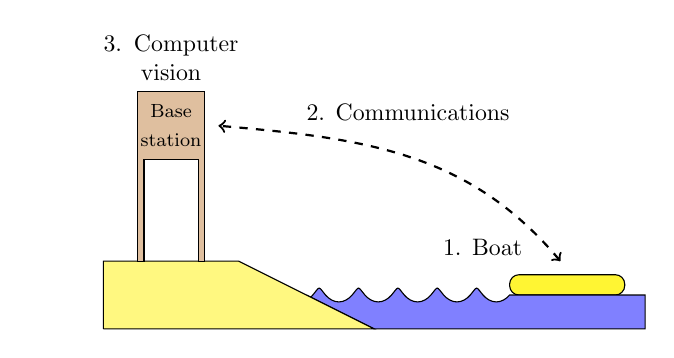
\begin{tikzpicture}[scale=0.86, every node/.style={transform shape}]
% Boat
\draw [fill=yellow!80, rounded corners=0.12cm] (6,0.5) rectangle (7.7,0.8);
% Landscape
\draw [fill=blue!50, decoration={coil, segment length=0.5cm}] (3,0.5) -- (4,0) -- (8,0) -- (8,0.5) -- (6,0.5) decorate { -- (2.5,0.5) };
\draw [fill=yellow!50] (0,0) -- (0,1) -- (2,1) -- (4,0) -- (0,0);
% Tower
\draw [fill=brown!50] (0.5,1) -- (0.5,3.5) -- (1.5,3.5) -- (1.5,1) -- (1.4,1) -- (1.4,2.5) -- (0.6,2.5) -- (0.6,1) -- (0.5,1);
% Comms
\draw [dashed, thick, out=130, in=-5, <->] (6.75,1) to (1.7,3);
% Labels
\draw (1,4) node [text width=4cm, align=center] {3. Computer\\vision};
\draw (4.5,3.2) node {2. Communications};
\draw (5.6,1.2) node {1. Boat};
\draw (1,3) node [text width=1cm, align=center] {\footnotesize Base\\station};
\end{tikzpicture}%
\hspace{0.1cm}%
% Boat overview
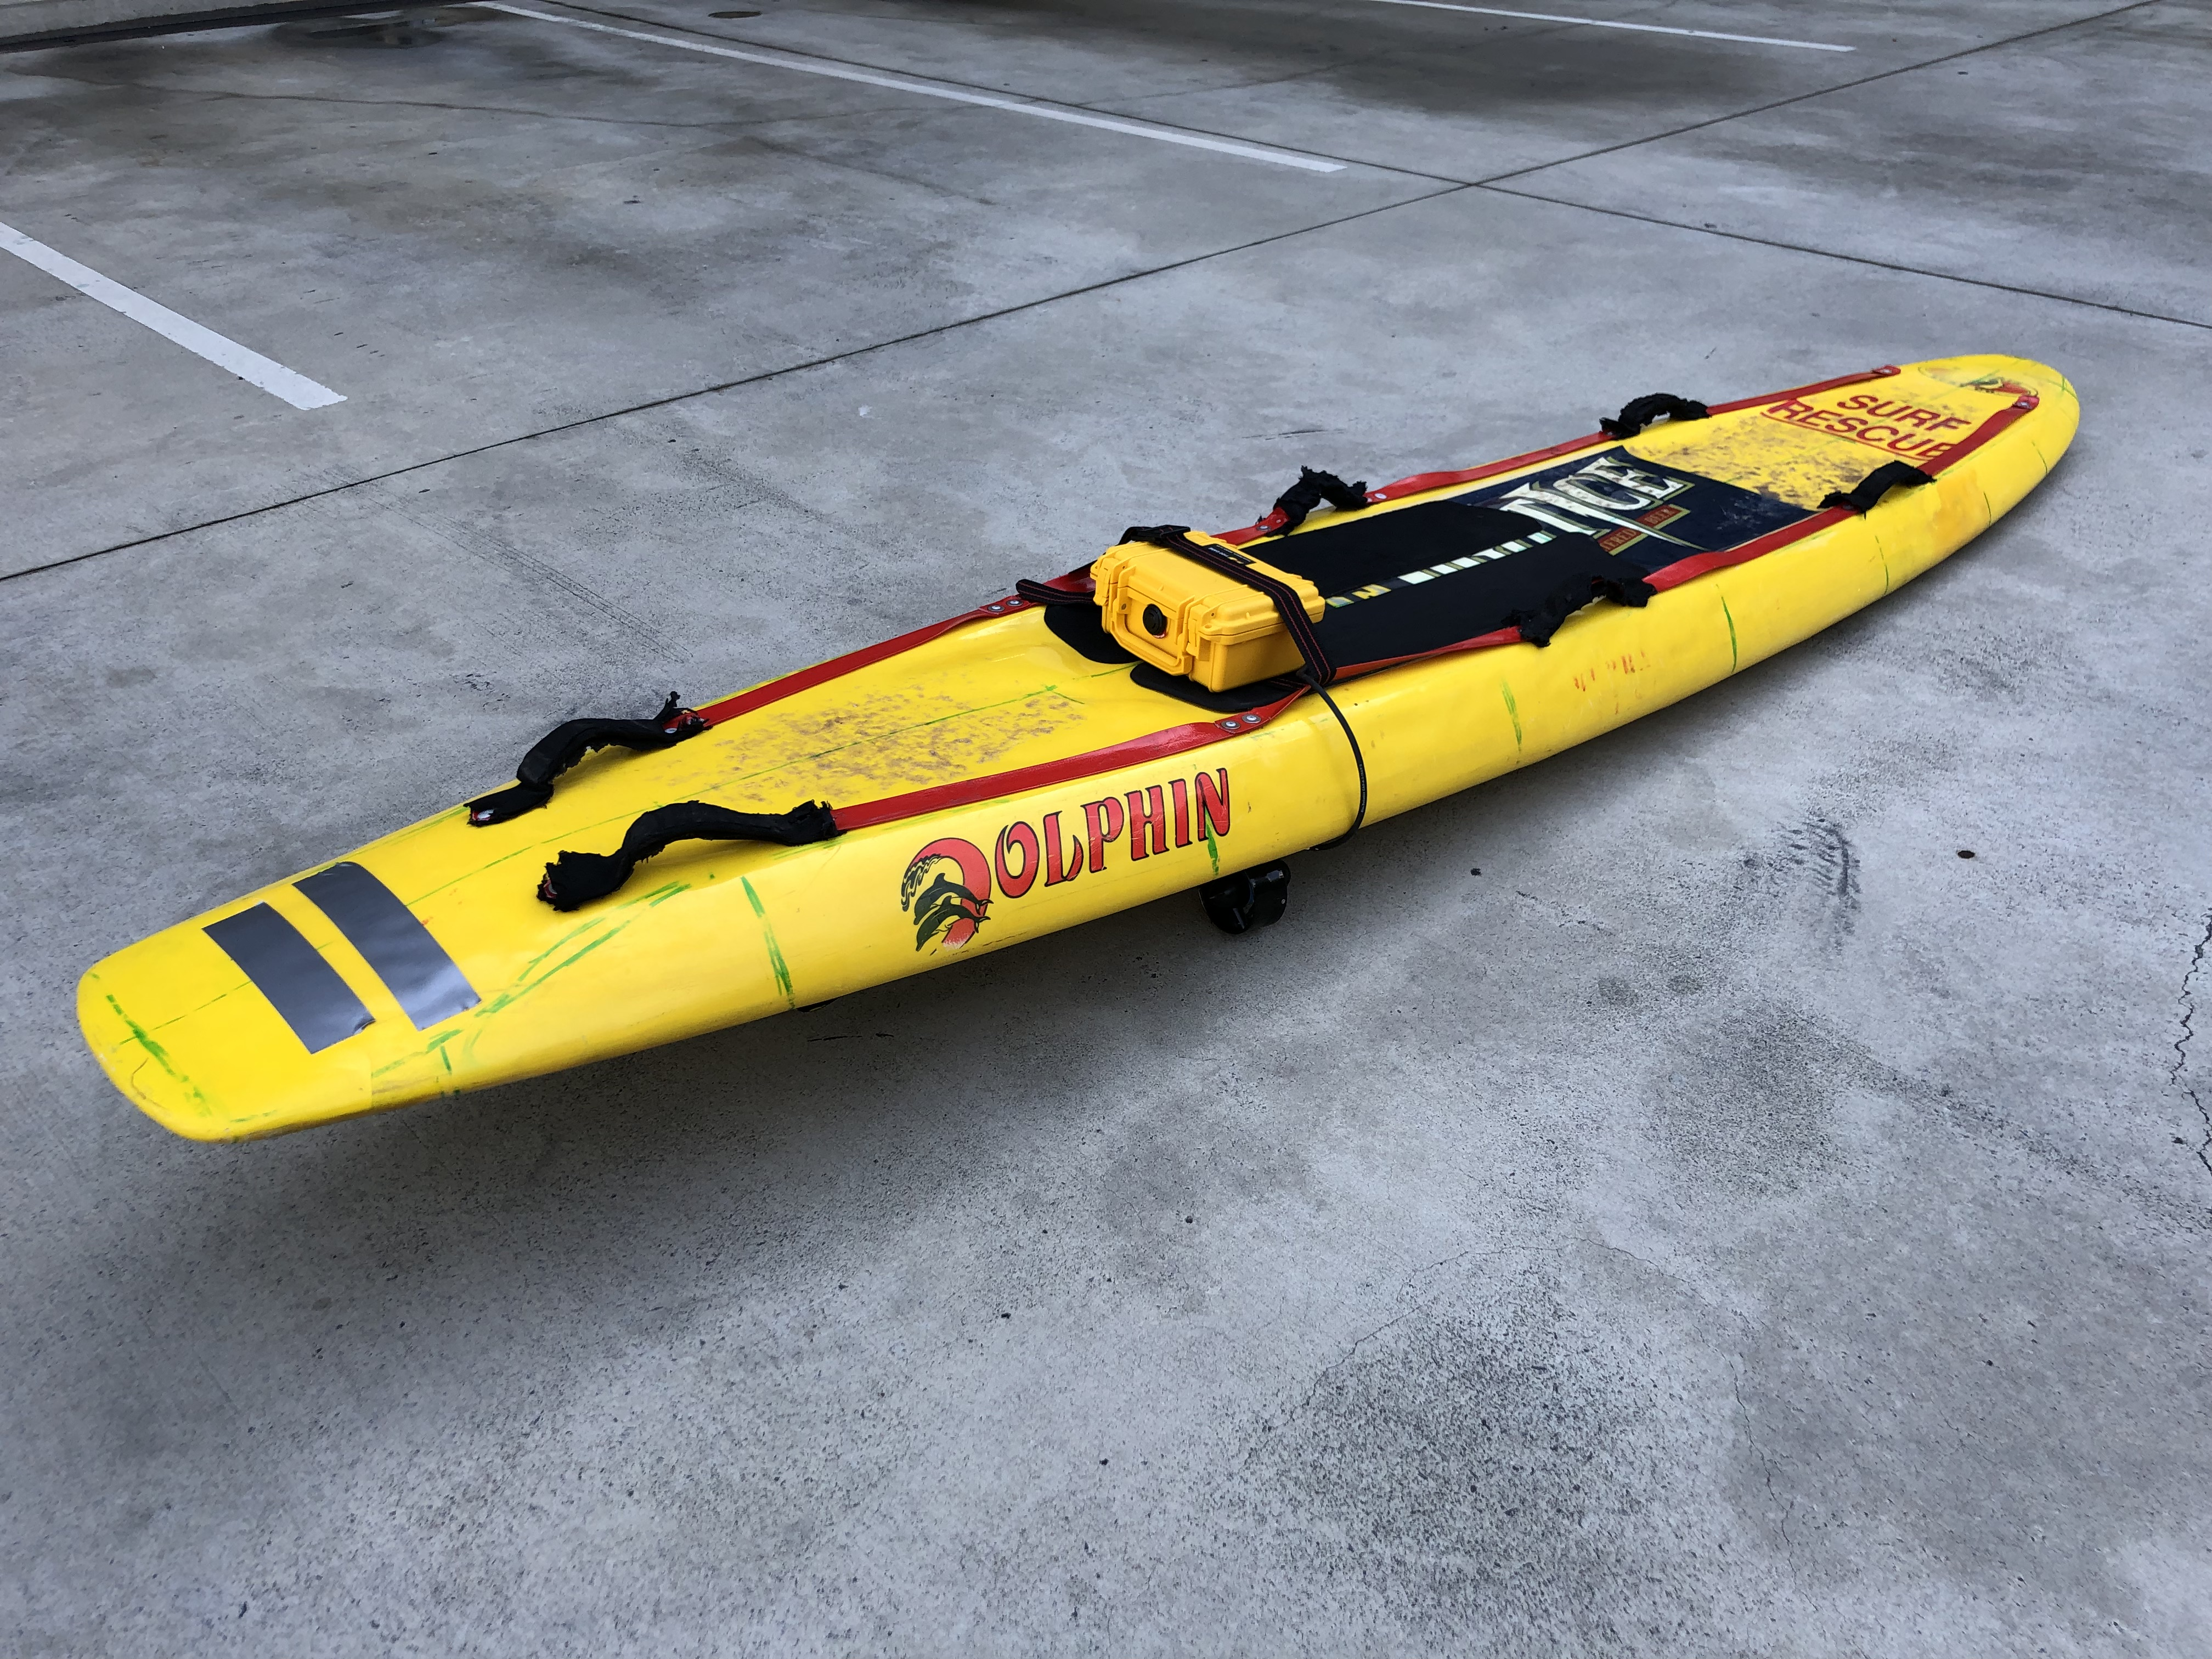
\includegraphics[height=0.4\textheight]{boat-overview.jpg}
\end{minipage}

% Row 2
\vspace{0.1cm}
\begin{minipage}{\textwidth}
\centering
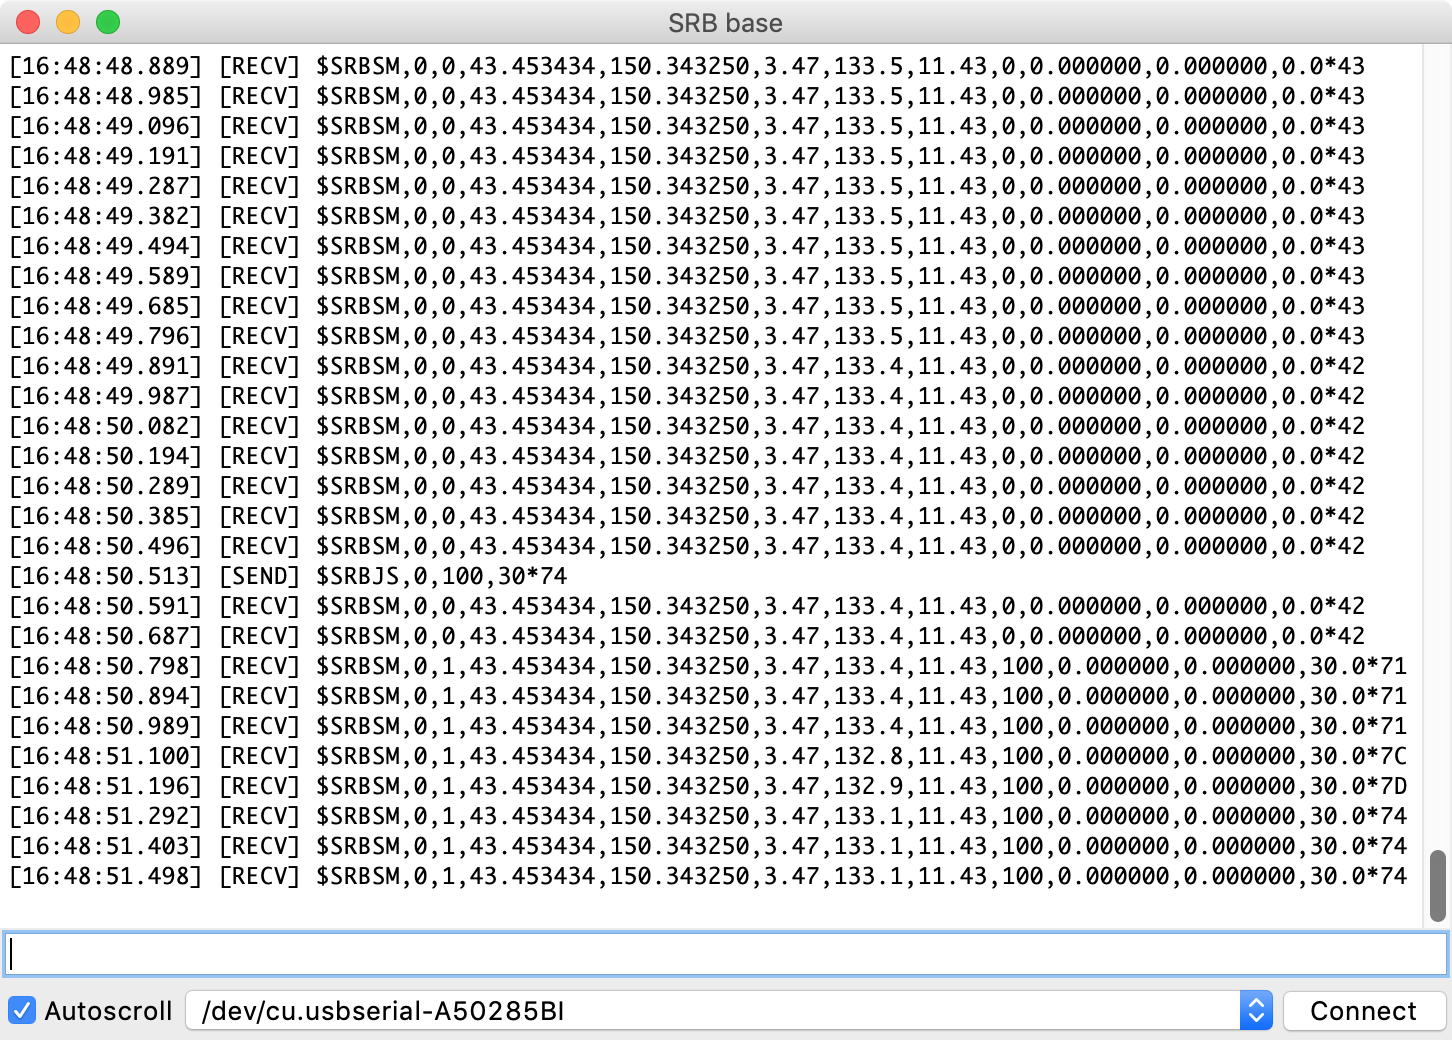
\includegraphics[height=0.34\textheight]{srb-base-screenshot.png}
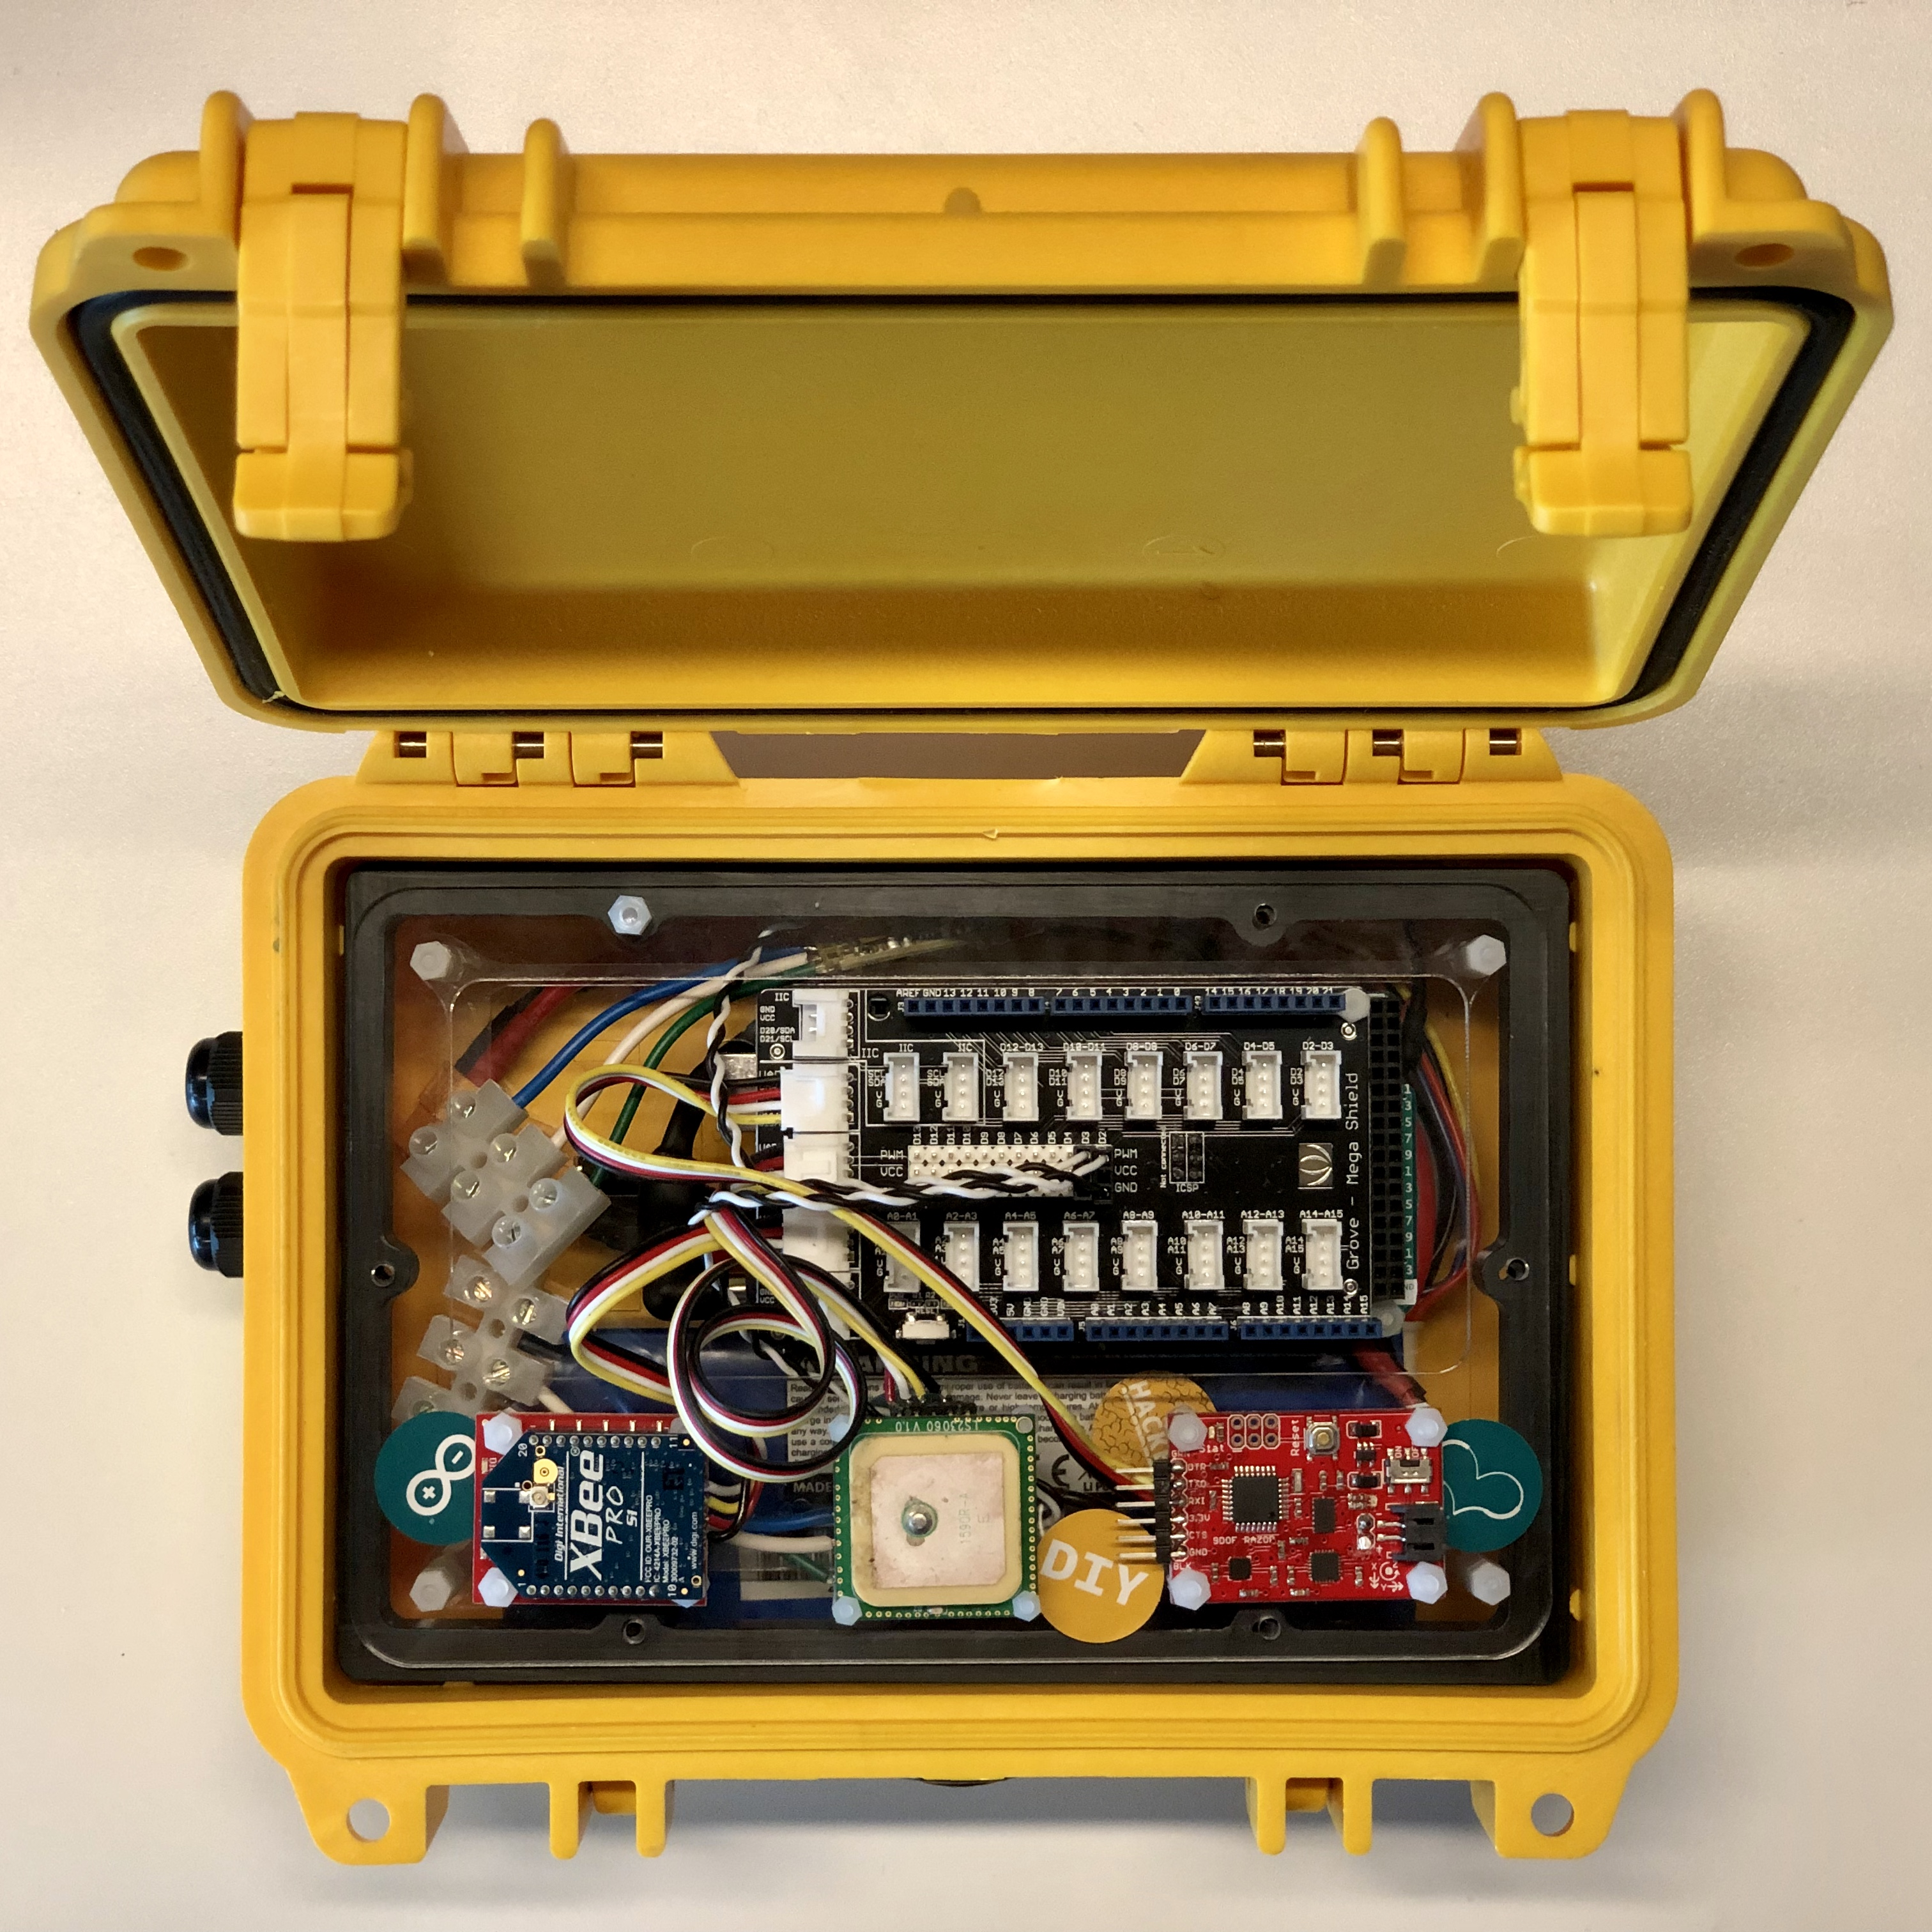
\includegraphics[height=0.34\textheight]{boat-hardware.jpg}
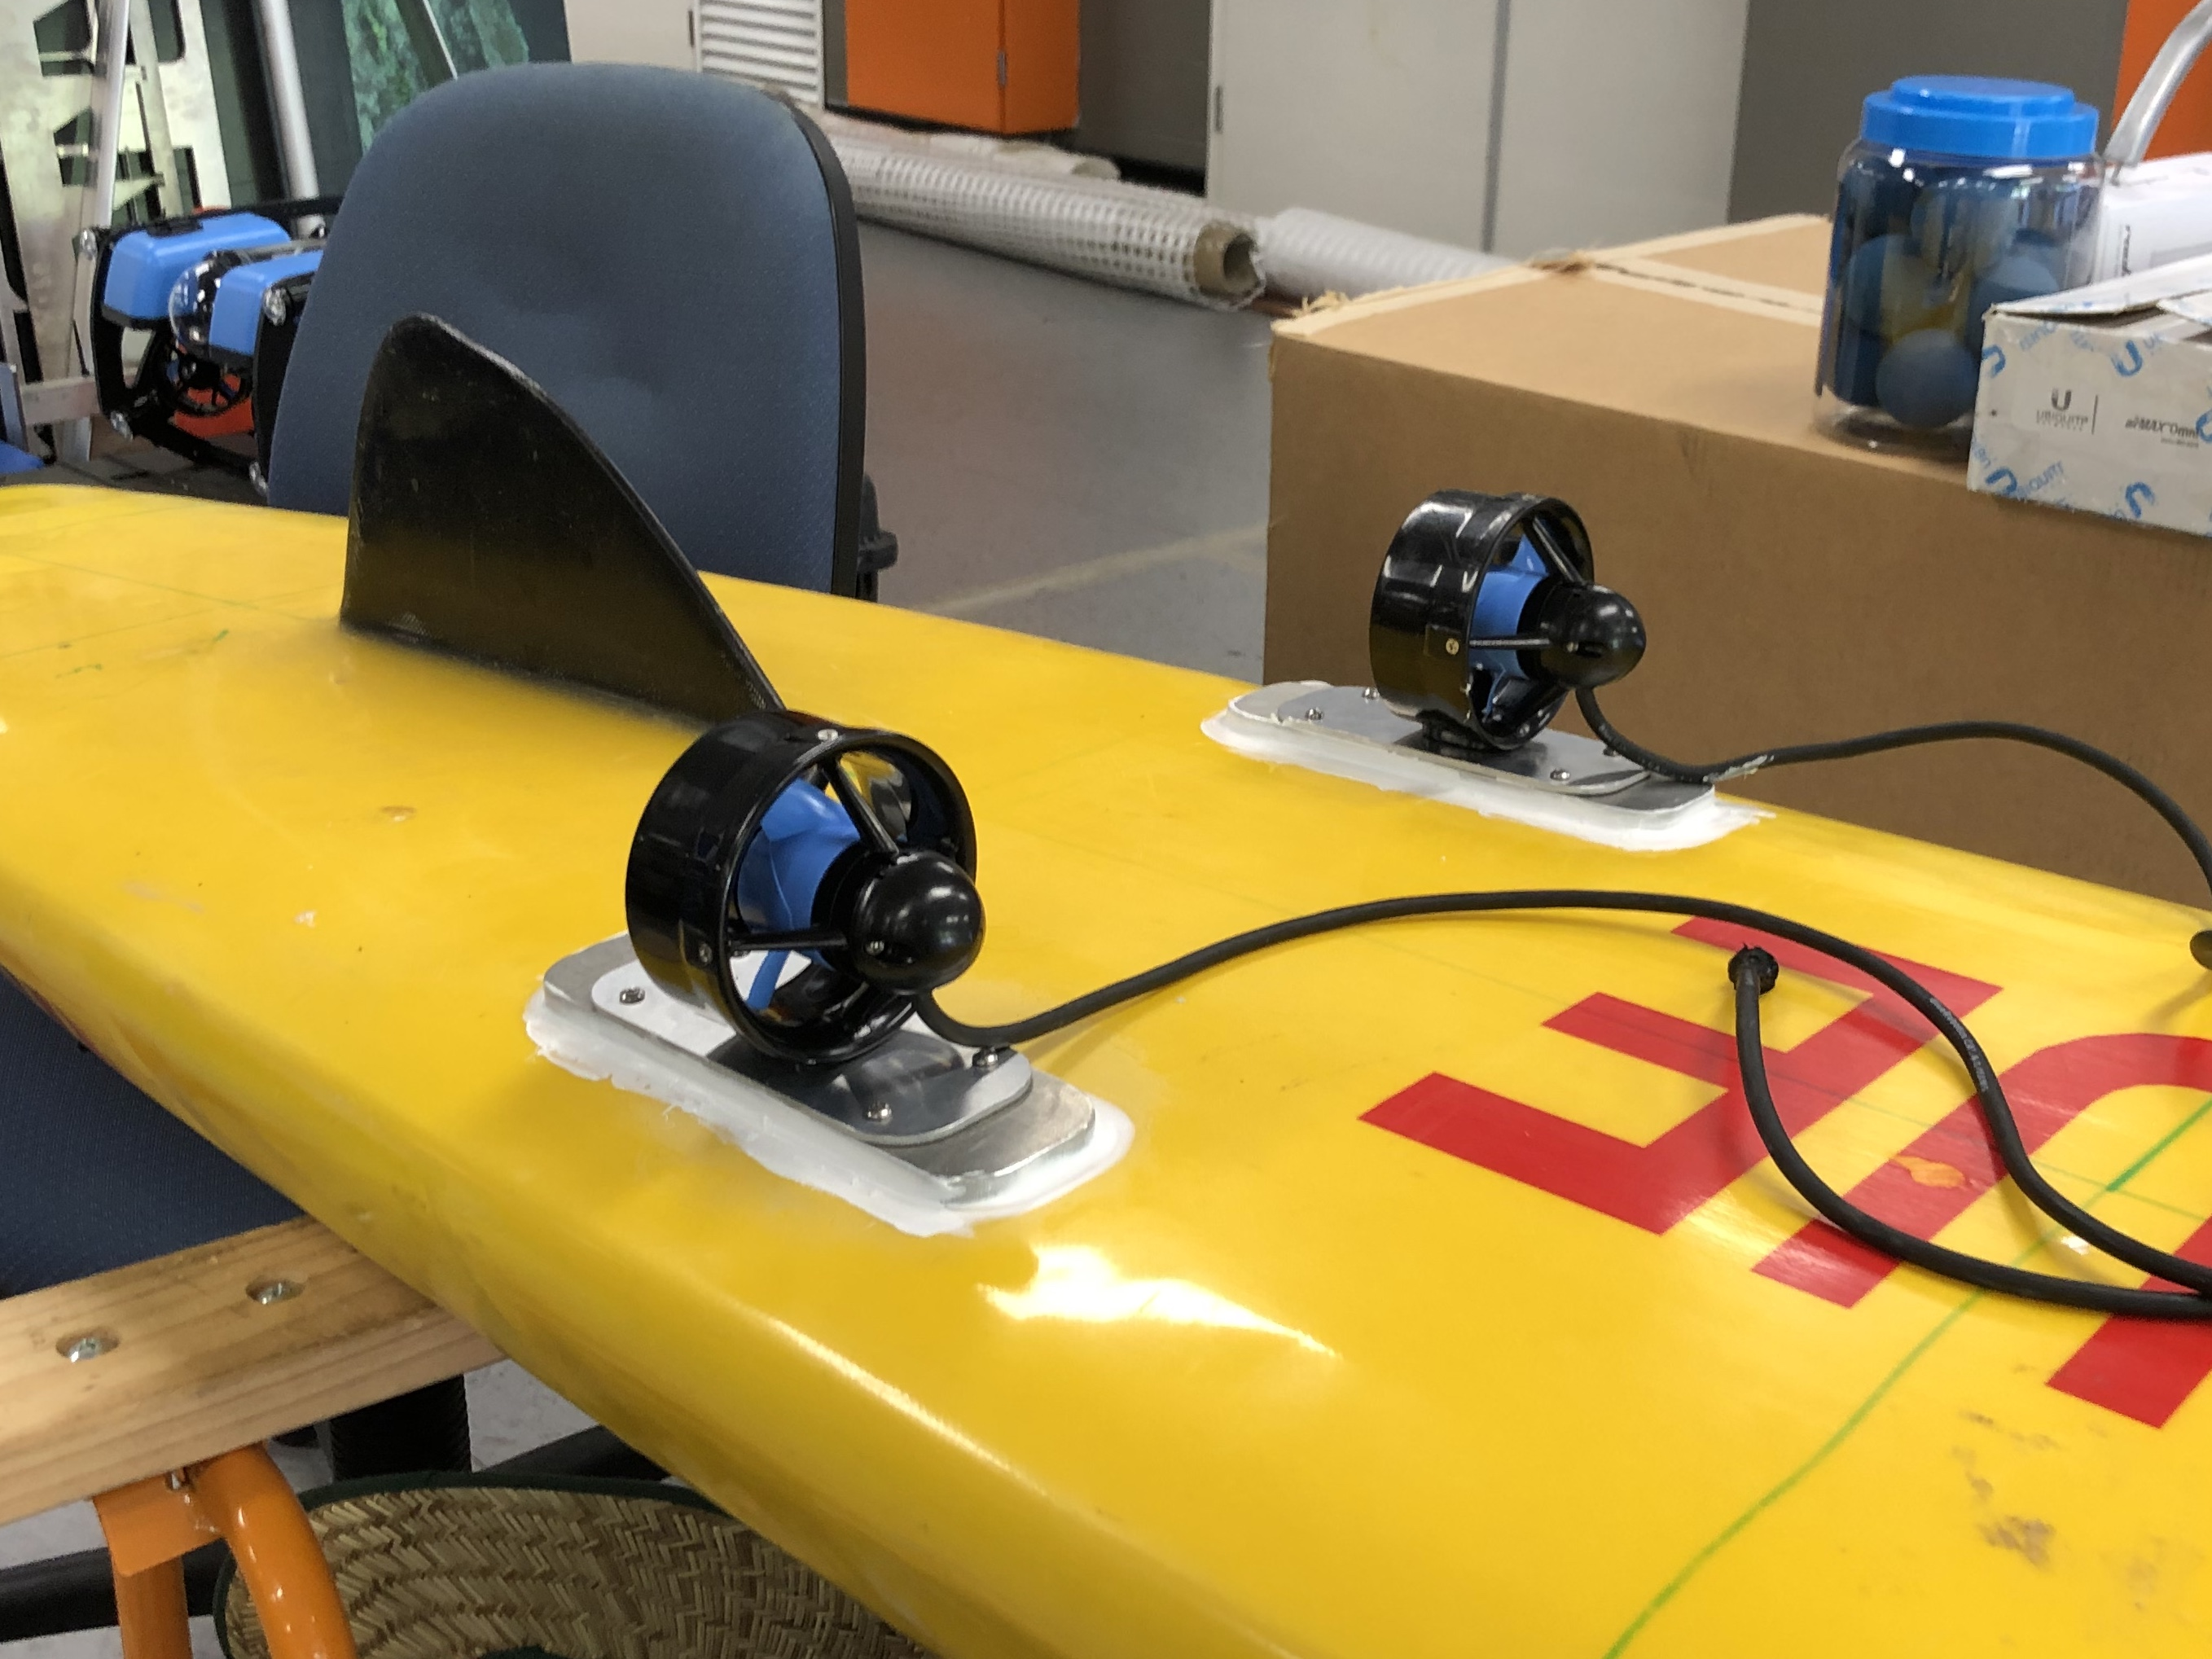
\includegraphics[height=0.34\textheight]{motors-mounted.jpg}
\end{minipage}

\end{frame}

\note{ \tiny

Life saving services rescue thousands of people every year and are essential to keeping public beaches safe. In Queensland alone, over three thousand are rescued and hundreds are resuscitated by lifesaving services every year. However, accidents can still happen and life savers are often required to place themselves at risk.

The Surf Rescue Boat system developed over the course of this project aims to supplement the work of life saving services at public beaches. The system comprises a semi-autonomous water vehicle (or the “boat”), a communications system, and a computer vision system as an interface for navigation.

As shown in the top-left diagram, the boat sits out in the calm ocean beyond the surf break of a beach. It communicates wirelessly with a base station on a lifeguard tower, where a live camera feed allows a user to pinpoint the target location of the boat in the surf, and a computer vision system translates this into GPS coordinates. The intended use case is for a life guard to send the boat to support a person in distress while they are being rescued.

On the underside of the boat, there are two powerful thrusters that provide propulsion and steering. These connect to a watertight box on the top side, which contains the boat's control electronics. The electronics are powered by lithium-polymer batteries, controlled by an Arduino Mega, obtains its bearings using a GPS receiver and inertial measurement unit, and communicates with the base station using an XBee radio.

A custom serial-based protocol was designed for communications and control. On the base station side, a utility was developed to send and receive formatted commands with error checking to and from the boat. Status messages are sent from the boat containing information like speed and position, and commands are sent from the base station that direct the boat through the surf.

In its current state, the Surf Rescue Boat is a very early prototype, and much more development is required, including the integration of the computer vision system. Testing was limited due to time constraints, but I intend to continue working on this project for a while and move it toward an operational system. In the future, the Surf Rescue Boat and similar systems could play an important role to help save countless lives in the surf along coastal public beaches.

}


\end{document}